\setcounter{ExampleCounter}{1}
\begin{center}
\includegraphics[width=0.8\textwidth]{Konigsberg_cropped}
\end{center}
In the early 1700s, the city of K\"onigsberg in Prussia (now Kaliningrad, Russia), which was split by the Pregel River, had 7 bridges connecting the north and south banks of the city to two islands in the center of the river, as shown in the drawing above.  A popular puzzle of the day challenged travelers to plan a walk through this part of the city in such a way that they would cross each bridge exactly once (you may want to pause and see if you can find such a path).

Leonhard Euler, in 1736, turned his attention to this problem.  Although the problem doesn't seem to be an important one, what is interesting is how Euler solved it.  He noticed that the path a person travels on a given land mass is irrelevant; all that matters is which bridges they cross.  Thus, he decided to simplify the picture by simply drawing a dot to represent each land mass, and a line connecting two dots to represent a bridge.  Here's the result:

\begin{center}
\begin{tikzpicture}
  \GraphInit[vstyle=simple]
  \tikzset{VertexStyle/.append style={scale=0.5}}
  \SetGraphUnit{1.4}
  \Vertex{1}
  \NOWE(1){2}
  \SOWE(1){4}
  \WE(1){3}
  \Edge(1)(2)
  \Edge(1)(3)
  \Edge(1)(4)
  \SetUpEdge[style={bend right=30}]
  \Edge(2)(3)
  \Edge(3)(4)
  \SetUpEdge[style={bend left=30}]
  \Edge(2)(3)
  \Edge(3)(4)
\end{tikzpicture}
\end{center}

That's the first example of a \textbf{graph}; while we use the word \emph{graph} to mean several different things, in this chapter, a graph will refer to a diagram like the one above.

\begin{formula}{Graphs}
A \textbf{graph}, in graph theory, consists of \textbf{nodes} (or vertices) and \textbf{edges}; each edge connects one node to another.
\end{formula}

Now, notice that we've drawn the nodes in positions that roughly correspond to the orientation of the map; the one on the right represents the eastern island, for instance, while the two on the top and bottom of the left row represent the northern and southern banks.

However,\marginnote{\emph{Location is not important.}\\ \text{}\\ \emph{Connections are what matters.}} this is completely arbitrary; since we simplified the picture to land masses and connections, it turns out that the nodes can be rearranged at will, as long as the final result has the same pattern of connections, meaning that the same nodes are connected by edges.
\pagebreak

Before we illustrate this, let's label each node so that we can see them move:

\begin{center}
\begin{tikzpicture}
  \SetGraphUnit{2}
  \Vertex{1}
  \NOWE(1){2}
  \SOWE(1){4}
  \WE(1){3}
  \Edge(1)(2)
  \Edge(1)(3)
  \Edge(1)(4)
  \SetUpEdge[style={bend right=30}]
  \Edge(2)(3)
  \Edge(3)(4)
  \SetUpEdge[style={bend left=30}]
  \Edge(2)(3)
  \Edge(3)(4)
\end{tikzpicture}
\end{center}

Each of these graphs is equivalent, according to Euler's new theory, to the original one:
\begin{center}
\begin{tabular}{c c c}
\begin{tikzpicture}
  \SetGraphUnit{1.5}
  \Vertex{1}
  \NO(1){2}
  \WE(1){4}
  \SOEA(1){3}
  \Edge(1)(2)
  \Edge(1)(3)
  \Edge(1)(4)
  %\SetUpEdge[style={bend right=30}]
  \Edge(2)(3)
  \Edge(3)(4)
  \SetUpEdge[style={bend left=30}]
  \Edge(2)(3)
  \Edge(3)(4)
\end{tikzpicture}
&
\begin{tikzpicture}
  \SetGraphUnit{1.5}
  \Vertex{1}
  \EA(1){2}
  \NOEA(1){4}
  \NOEA(4){3}
  \Edge(1)(2)
  \Edge(1)(4)
  \SetUpEdge[style={bend right=40}]
  \Edge(2)(3)
  \Edge(3)(4)
  \SetUpEdge[style={bend right=20}]
  \Edge(1)(3)
  \Edge(2)(3)
  \Edge(3)(4)
\end{tikzpicture}
&
\begin{tikzpicture}
  \SetGraphUnit{2.5}
  \Vertex{1}
  \SOWE(1){2}
  \WE(1){4}
  \SO(1){3}
  \Edge(1)(2)
  \Edge(1)(3)
  \Edge(1)(4)
  \Edge(2)(3)
  \Edge(3)(4)
  \SetUpEdge[style={bend right=30}]
  \Edge(2)(3)
  \Edge(3)(4)
\end{tikzpicture}
\end{tabular}
\end{center}

In fact, we could describe it in words,\marginnote{Of course, it's much more fun to draw pictures than to write something like this.} by saying something like
\begin{center}
There are 4 nodes.\\
Node 1 is connected to nodes 2, 3, and 4.\\
Node 2 is connected to node 3 by two edges.\\
Node 3 is connected to node 4 by two edges.
\end{center}
Any picture you could draw that fits this description would be equivalent to the first graph that we drew.

\subsection{Examples and Definitions}
Let's take a look at a few examples of graphs, and along the way, we'll encounter a few new terms that we can use to categorize and describe them.

\paragraph{Transportation Network}\marginnote{\textbf{Application 1}} The graph below shows a simple train system; each edge indicates a line that runs between two cities.

\begin{center}
\begin{tikzpicture}[scale=0.75]
  \GraphInit[vstyle=simple]
  \tikzset{VertexStyle/.append style={scale=0.5}}
  \Vertex[x=0,y=0]{DC}
  \extralabel[2mm]{DC}{-90}{DC}
  \Vertex[x=-2,y=2]{Pitt}
  \extralabel[2mm]{Pitt}{180}{Pittsburgh}
  \Vertex[x=2,y=3]{NYC}
  \extralabel[2mm]{NYC}{-30}{New York}
  \Vertex[x=4,y=4]{Boston}
  \extralabel[2mm]{Boston}{0}{Boston}
  \Edge(DC)(Pitt)
  \Edge(DC)(NYC)
  \Edge(Pitt)(NYC)
  \Edge(NYC)(Boston)
  \Loop[dist=1.5cm,dir=NO,style={-}](NYC)
\end{tikzpicture}
\end{center}

Notice the \textbf{loop} at New York; this implies that there is a train line that returns to the same station from which it leaves.  There could be, for instance, a sightseeing train that simply takes passengers on a short loop.  We simply include it here to show the possibility of a loop, which is an edge that connects a node to itself.
\pagebreak

\paragraph{Communication Network}\marginnote{\textbf{Application 2}} This second example shows a fictional network, which could consist of connections between data centers.

\begin{center}
\begin{tikzpicture}[scale=1]
  \GraphInit[vstyle=simple]
  \tikzset{VertexStyle/.append style={scale=0.5}}
  \Vertex[x=0,y=0]{SF}
  \extralabel[2mm]{SF}{90}{San Francisco}
  \Vertex[x=1,y=-1]{LA}
  \extralabel[2mm]{LA}{-90}{Los Angeles}
  \Vertex[x=3,y=-0.3]{Denver}
  \extralabel[2mm]{Denver}{-30}{Denver}
  \Vertex[x=5,y=0.3]{Chicago}
  \extralabel[2mm]{Chicago}{130}{Chicago}
  \Vertex[x=6,y=1]{Detroit}
  \extralabel[2mm]{Detroit}{90}{Detroit}
  \Vertex[x=7.5,y=0]{DC}
  \extralabel[2mm]{DC}{-90}{DC}
  \Vertex[x=8,y=0.8]{NY}
  \extralabel[2mm]{NY}{0}{New York}
  
  \tikzset{EdgeStyle/.style = {->-,>=latex[round]}}
  \Edge(SF)(LA)
  \Edge(SF)(Denver)
  \Edge(NY)(Chicago)
  \Edge(DC)(NY)
  \Edge(Chicago)(Detroit)
  \Edge(Detroit)(NY)
  
  \tikzset{EdgeStyle/.style = {->-,>=latex[round],bend right=10}}
  \Edge(LA)(Denver)
  \Edge(Denver)(Chicago)
  \Edge(Chicago)(DC)
  
  \Edge(Denver)(LA)
  \Edge(Chicago)(Denver)
  \Edge(DC)(Chicago)
\end{tikzpicture}
\end{center}

Notice that the edges on this graph have arrows that indicate which direction the data can travel; for instance, data can flow from Detroit to New York, but to send data in the opposite direction, it would have to go from New York to Chicago, and then on to Detroit.

Also, this graph, unlike the one before it, has multiple edges between some pairs of nodes (we've seen this before, on the graph of K\"onigsberg).

These two distinctions lead to our first set of definitions; the following terms can help to categorize graphs, and it is useful to think about new applications in terms of what category they fit into.

\begin{formula}{Graph Classifications}
\textbf{Simple Graphs and Multigraphs:} a \textbf{simple graph} is one that has at most one edge between two nodes, and contains no loops; a \textbf{multigraph} can have multiple edges connecting the same pair of nodes, and may contain loops.\\

\textbf{Undirected and Directed Graphs:} an \textbf{undirected graph} has no notion of direction to the edges; in a \textbf{directed graph} (also called a \textbf{digraph}), each edge has an associated direction.
\end{formula}

\begin{example}[https://www.youtube.com/watch?v=4Q8wrqaKKDE&list=PLfmpjsIzhztst_PxJXo574wshSwxU9Yg_&index=1]{Classifying Graphs}
For each of the following graphs, determine whether it is a simple graph or multigraph, and whether it is directed or undirected.

\begin{center}
\begin{tabular}{c c c c}
\begin{tikzpicture}
  \GraphInit[vstyle=simple]
  \tikzset{VertexStyle/.append style={scale=0.3}}
  \SetGraphUnit{1}
  \tikzset{EdgeStyle/.style = {->-,>=latex[round]}}
  \Vertex{1}
  \NO(1){2}
  \EA(1){3}
  \NO(3){4}
  \EA(3){5}
  \Edge(1)(2)
  \Edge(1)(3)
  \Edge(1)(4)
  \Edge(4)(2)
  \Edge(3)(4)
  \Edge(5)(3)
  \tikzset{EdgeStyle/.style = {->-,>=latex[round],bend right=20}}
  \Edge(5)(4)
  \Edge(4)(5)
\end{tikzpicture}
&
\begin{tikzpicture}
  \GraphInit[vstyle=simple]
  \tikzset{VertexStyle/.append style={scale=0.3}}
  \SetGraphUnit{1}
  \Vertex{1}
  \NO(1){2}
  \EA(2){3}
  \NO(3){4}
  \EA(4){5}
  \Edge(1)(2)
  \Edge(1)(3)
  \Edge(2)(3)
  \Edge(2)(4)
  \Edge(3)(4)
  \Edge(4)(5)
\end{tikzpicture}
&
\begin{tikzpicture}
  \GraphInit[vstyle=simple]
  \tikzset{VertexStyle/.append style={scale=0.3}}
  \SetGraphUnit{1}
  \Vertex{1}
  \NOWE(1){2}
  \SetUpEdge[style={bend right=30}]
  \Edge(1)(2)
  \Edge(2)(1)
  \Loop[dist=1cm,dir=NO,style={-,line width=0.7pt}](2)
\end{tikzpicture}
&
\begin{tikzpicture}
  \GraphInit[vstyle=simple]
  \tikzset{VertexStyle/.append style={scale=0.3}}
  \SetGraphUnit{1}
  \tikzset{EdgeStyle/.style = {->-,>=latex[round]}}
  \Vertex{1}
  \NOWE(1){2}
  \NOEA(1){3}
  \NOEA(2){4}
  \Edge(1)(2)
  \Edge(1)(3)
  \Edge(4)(1)
  \Edge(4)(2)
  \Edge(3)(4)
\end{tikzpicture}\\
& & & \\
(a) & (b) & (c) & (d)
\end{tabular}
\end{center}

\sol
\begin{enumerate}[(a)]
\item Since the edges have directions associated with them, and there is one pair of nodes that have multiple edges between them, this is a \boxtext{directed multigraph}
\item There are no multiple edges or loops, and no directions, so this is an \boxtext{undirected simple graph}
\item There are no arrows, but because of the multiple edges and the loop, this is an \boxtext{undirected multigraph}
\item There are no multiple edges or loops, so this one is simple, but because of the arrows, it is a \boxtext{directed simple graph}
\end{enumerate}
\end{example}
\pagebreak

Let's go back to examples of graph theory applications.

\paragraph{Social Network}\marginnote{\textbf{Application 3}} Suppose, for instance, that we selected a small group of people and checked whether they are connected on Facebook; if two people are friends, we draw an edge between them.
\begin{center}
\begin{tikzpicture}[scale=2]
  \GraphInit[vstyle=simple]
  \tikzset{VertexStyle/.append style={scale=0.5}}
  \Vertex{Agnes}
  \NO(Agnes){Ellis}
  \EA(Agnes){Marie}
  \NO(Marie){Ivan}
  \NO(Ivan){Tamara}
  \WE(Tamara){Joel}
  \EA(Marie){Musa}
  \EA(Ivan){Kira}
  \extralabel[1mm]{Agnes}{225}{Agnes}
  \extralabel[1mm]{Ellis}{180}{Ellis}
  \extralabel[1mm]{Marie}{-90}{Marie}
  \extralabel[1mm]{Ivan}{45}{Ivan}
  \extralabel[1mm]{Tamara}{45}{Tamara}
  \extralabel[1mm]{Joel}{135}{Joel}
  \extralabel[1mm]{Musa}{-45}{Musa}
  \extralabel[1mm]{Kira}{0}{Kira}
  \Edge(Agnes)(Ellis)
  \Edge(Agnes)(Ivan)
  \Edge(Ivan)(Marie)
  \Edge(Ivan)(Joel)
  \Edge(Joel)(Tamara)
  \Edge(Tamara)(Kira)
  \Edge(Kira)(Marie)
  \Edge(Ivan)(Musa)
  \Edge(Ellis)(Tamara)
  \SetUpEdge[style={bend right=10}]
  \Edge(Musa)(Tamara)
  \Edge(Joel)(Musa)
\end{tikzpicture}
\end{center}

This is a simple graph, since it doesn't make sense to have more than one connection between two people; they are either friends or are not.  Also, since Facebook friendship is a two-way relationship, this is an undirected graph.

If we wanted to make a directed multigraph for a social network, we could use Instagram, for instance, since one person can follow another without being followed back.  The result might look like this:\marginnote{\emph{Notice how complicated this is already, with only 8 people.  Real social networks have incredibly complicated graphs; although we may not be able to draw them, computers can still analyze them to glean all sorts of information, like which users are the most influential.}}
\begin{center}
\begin{tikzpicture}[scale=2]
  \GraphInit[vstyle=simple]
  \tikzset{VertexStyle/.append style={scale=0.5}}
  \Vertex{Agnes}
  \NO(Agnes){Ellis}
  \EA(Agnes){Marie}
  \NO(Marie){Ivan}
  \NO(Ivan){Tamara}
  \WE(Tamara){Joel}
  \EA(Marie){Musa}
  \EA(Ivan){Kira}
  \extralabel[1mm]{Agnes}{225}{Agnes}
  \extralabel[1mm]{Ellis}{180}{Ellis}
  \extralabel[1mm]{Marie}{-90}{Marie}
  \extralabel[1mm]{Ivan}{-45}{Ivan}
  \extralabel[1mm]{Tamara}{45}{Tamara}
  \extralabel[1mm]{Joel}{135}{Joel}
  \extralabel[1mm]{Musa}{-45}{Musa}
  \extralabel[1mm]{Kira}{0}{Kira}
  
  \tikzset{EdgeStyle/.style = {->-,>=latex[round]}}
  \Edge(Joel)(Ellis)
  \Edge(Ivan)(Agnes)
  \Edge(Musa)(Kira)
  \tikzset{EdgeStyle/.style = {->-,>=latex[round],bend right=20}}
  \Edge(Agnes)(Ellis)
  \Edge(Ellis)(Agnes)
  \Edge(Joel)(Musa)
  \Edge(Musa)(Joel)
  \Edge(Marie)(Ivan)
  \Edge(Ivan)(Marie)
  \Edge(Kira)(Tamara)
  \Edge(Tamara)(Kira)
  \Edge(Ellis)(Tamara)
  \Edge(Tamara)(Ellis)
\end{tikzpicture}
\end{center}

Here, an edge indicates whether one person follows another, and the direction of the arrow goes from the follower to the one they follow.\\

Notice that one of the things we can glean from a graph like these is who in this social group is the most well-connected.  The easiest way to do this is simply to count the number of connections that each person has to others, which corresponds to the number of edges that connect to that node.  We have a special name for this count: we call it the \textbf{degree} of a node.

\begin{formula}{Degree}
The \textbf{degree} of a node in an undirected graph is the number of edges that connect to it.\\

\emph{Note: a loop counts twice, since the loop connects to the node at both of its ends.  This is mostly by convention, but it is important so that some concepts are consistent whether loops are included or not.}\\

In a directed graph, each node has two degrees: the \textbf{in-degree} and \textbf{out-degree}.  The in-degree counts how many edges come into that node; the out-degree counts how many edges leave from that node.
\end{formula}
\pagebreak

\begin{example}[https://www.youtube.com/watch?v=ppDOCfP0lYs&list=PLfmpjsIzhztst_PxJXo574wshSwxU9Yg_&index=2]{Degrees of Nodes}
Find the degree of each node in the social network graphs shown here.
\begin{center}
\begin{tabular}{c c}
\begin{tikzpicture}[scale=1.5]
  \GraphInit[vstyle=simple]
  \tikzset{VertexStyle/.append style={scale=0.5}}
  \Vertex{Agnes}
  \NO(Agnes){Ellis}
  \EA(Agnes){Marie}
  \NO(Marie){Ivan}
  \NO(Ivan){Tamara}
  \WE(Tamara){Joel}
  \EA(Marie){Musa}
  \EA(Ivan){Kira}
  %\extralabel[1mm]{Agnes}{225}{Agnes}
  %\extralabel[1mm]{Ellis}{180}{Ellis}
  %\extralabel[1mm]{Marie}{-90}{Marie}
  %\extralabel[0.25mm]{Ivan}{80}{Ivan}
  %\extralabel[1mm]{Tamara}{45}{Tamara}
  %\extralabel[1mm]{Joel}{135}{Joel}
  %\extralabel[1mm]{Musa}{-45}{Musa}
  %\extralabel[1mm]{Kira}{0}{Kira}
  \Edge(Agnes)(Ellis)
  \Edge(Agnes)(Ivan)
  \Edge(Ivan)(Marie)
  \Edge(Ivan)(Joel)
  \Edge(Joel)(Tamara)
  \Edge(Tamara)(Kira)
  \Edge(Kira)(Marie)
  \Edge(Ivan)(Musa)
  \Edge(Ellis)(Tamara)
  \SetUpEdge[style={bend right=15}]
  \Edge(Musa)(Tamara)
  \Edge(Joel)(Musa)
  \Loop[dist=1cm,dir=NOEA,style={-,line width=0.7pt}](Musa)
\end{tikzpicture}
\hspace*{0.25in}
&
\hspace*{0.25in}
\begin{tikzpicture}[scale=1.5]
  \GraphInit[vstyle=simple]
  \tikzset{VertexStyle/.append style={scale=0.5}}
  \Vertex{Agnes}
  \NO(Agnes){Ellis}
  \EA(Agnes){Marie}
  \NO(Marie){Ivan}
  \NO(Ivan){Tamara}
  \WE(Tamara){Joel}
  \EA(Marie){Musa}
  \EA(Ivan){Kira}
  %\extralabel[1mm]{Agnes}{225}{Agnes}
  %\extralabel[1mm]{Ellis}{180}{Ellis}
  %\extralabel[1mm]{Marie}{-90}{Marie}
  %\extralabel[0.25mm]{Ivan}{92}{Ivan}
  %\extralabel[1mm]{Tamara}{45}{Tamara}
  %\extralabel[1mm]{Joel}{135}{Joel}
  %\extralabel[1mm]{Musa}{-45}{Musa}
  %\extralabel[1mm]{Kira}{0}{Kira}
  
  \tikzset{EdgeStyle/.style = {->-,>=latex[round]}}
  \Edge(Joel)(Ellis)
  \Edge(Ivan)(Agnes)
  \Edge(Musa)(Kira)
  \Loop[dist=0.5cm,dir=NOEA,style={-,line width=0.7pt}](Musa)
  \tikzset{EdgeStyle/.style = {->-,>=latex[round],bend right=20}}
  \Edge(Agnes)(Ellis)
  \Edge(Ellis)(Agnes)
  \Edge(Marie)(Ivan)
  \Edge(Ivan)(Marie)
  \Edge(Kira)(Tamara)
  \Edge(Tamara)(Kira)
  \Edge(Ellis)(Tamara)
  \Edge(Tamara)(Ellis)
\end{tikzpicture}\\
& \\
(a) \hspace*{0.25in} & \hspace*{0.25in} (b)
\end{tabular}
\end{center}

\sol
We simply need to count the number of edges that connect at each node.  The only complication in part (a) is the loop on the lower-right node; remember that the loop adds a total of 2 the degree of that node.  For part (b), pay attention to the direction of each edge; an edge adds one to the out-degree of its starting node and one to the in-degree of its ending node (note that a loop here contributes one each to the in-degree and out-degree of its node).\\

Here's the final result; each node is labeled with its degree(s):
\begin{center}
\begin{tabular}{c c}
\begin{tikzpicture}[scale=1.25]
  \GraphInit[vstyle=simple]
  \tikzset{VertexStyle/.append style={scale=0.5}}
  \Vertex{Agnes}
  \NO(Agnes){Ellis}
  \EA(Agnes){Marie}
  \NO(Marie){Ivan}
  \NO(Ivan){Tamara}
  \WE(Tamara){Joel}
  \EA(Marie){Musa}
  \EA(Ivan){Kira}
  \extralabel[1mm]{Agnes}{225}{\Large\color{red!80!black}2}
  \extralabel[1mm]{Ellis}{180}{\Large\color{red!80!black}2}
  \extralabel[1mm]{Marie}{-90}{\Large\color{red!80!black}2}
  \extralabel[0.25mm]{Ivan}{80}{\Large\color{red!80!black}4}
  \extralabel[1mm]{Tamara}{45}{\Large\color{red!80!black}4}
  \extralabel[1mm]{Joel}{135}{\Large\color{red!80!black}3}
  \extralabel[1mm]{Musa}{-45}{\Large\color{red!80!black}5}
  \extralabel[1mm]{Kira}{0}{\Large\color{red!80!black}2}
  \Edge(Agnes)(Ellis)
  \Edge(Agnes)(Ivan)
  \Edge(Ivan)(Marie)
  \Edge(Ivan)(Joel)
  \Edge(Joel)(Tamara)
  \Edge(Tamara)(Kira)
  \Edge(Kira)(Marie)
  \Edge(Ivan)(Musa)
  \Edge(Ellis)(Tamara)
  \SetUpEdge[style={bend right=15}]
  \Edge(Musa)(Tamara)
  \Edge(Joel)(Musa)
  \Loop[dist=1cm,dir=NOEA,style={-,line width=0.7pt}](Musa)
\end{tikzpicture}
&
\begin{tikzpicture}[scale=1.75]
  \GraphInit[vstyle=simple]
  \tikzset{VertexStyle/.append style={scale=0.5}}
  \Vertex{Agnes}
  \NO(Agnes){Ellis}
  \EA(Agnes){Marie}
  \NO(Marie){Ivan}
  \NO(Ivan){Tamara}
  \WE(Tamara){Joel}
  \EA(Marie){Musa}
  \EA(Ivan){Kira}
  \extralabel[1mm]{Agnes}{225}{\color{red!80!black}\parbox{1.5cm}{\centering In: 2\\ Out: 1}}
  \extralabel[1mm]{Ellis}{180}{\color{red!80!black}\parbox{1.5cm}{\centering In: 3\\ Out: 2}}
  \extralabel[1mm]{Marie}{-90}{\color{red!80!black}\parbox{1.5cm}{\centering In: 1\\ Out: 1}}
  \extralabel[0.25mm]{Ivan}{92}{\color{red!80!black}\parbox{1.5cm}{\centering In: 1\\ Out: 2}}
  \extralabel[1mm]{Tamara}{45}{\color{red!80!black}\parbox{1.5cm}{\centering In: 2\\ Out: 2}}
  \extralabel[1mm]{Joel}{135}{\color{red!80!black}\parbox{1.5cm}{\centering In: 0\\ Out: 1}}
  \extralabel[1mm]{Musa}{-45}{\color{red!80!black}\parbox{1.5cm}{\centering In: 1\\ Out: 2}}
  \extralabel[1mm]{Kira}{0}{\color{red!80!black}\parbox{1.5cm}{\centering In: 2\\ Out: 1}}
  
  \tikzset{EdgeStyle/.style = {->-,>=latex[round]}}
  \Edge(Joel)(Ellis)
  \Edge(Ivan)(Agnes)
  \Edge(Musa)(Kira)
  \Loop[dist=0.5cm,dir=NOEA,style={-,line width=0.7pt}](Musa)
  \tikzset{EdgeStyle/.style = {->-,>=latex[round],bend right=20}}
  \Edge(Agnes)(Ellis)
  \Edge(Ellis)(Agnes)
  \Edge(Marie)(Ivan)
  \Edge(Ivan)(Marie)
  \Edge(Kira)(Tamara)
  \Edge(Tamara)(Kira)
  \Edge(Ellis)(Tamara)
  \Edge(Tamara)(Ellis)
\end{tikzpicture}\\
& \\
(a) & (b)
\end{tabular}
\end{center}
\end{example}

There are a couple of interesting observations we can make about node degrees.

\begin{formula}{Degrees: Observation 1}
The sum of the degrees of all the nodes in an undirected graph is always even.\\

Similarly, the sum of all in-degrees and out-degrees of all the nodes in a directed graph is always even.
\end{formula}

The reason for this is very simple: each edge contributes two degrees to the total for the graph, one degree at each end, so no matter how many edges there are, there will be twice as many degrees, and two times anything is always even.  In a directed graph, each edge contributes one out-degree and one in-degree; thus, the total in-degrees and out-degrees will be equal, and when these are added, the result will also be even.

\begin{formula}{Degrees: Observation 2}
An undirected graph has an even number of nodes with odd degree.
\end{formula}
\pagebreak
\text{}
\vfill

To verify this, we need to remember that the total number of degrees is even, and we need to know a principle of even numbers: \textbf{if you start with an even number, add something to it, and end up with an even number, the number you added must have been even}.  In other words, if you add an even number and an odd number, the result will be odd.

Therefore, if we split the graph into even nodes and odd nodes, we can split up the total of all degrees (which we know is even) like this:
\begin{center}
degrees of even nodes $+$ degrees of odd nodes $=$ even
\end{center}
Since the first part is even (if you add up a bunch of even degrees, the result is even), and the result is even, we know that the total number of degrees for all the odd nodes must be even also (that's the bolded principle in the last paragraph).

Think about adding together a bunch of odd numbers: when we add two of them, we get an even result, but adding a third makes the result odd.  Adding a fourth makes it even again, and so on, so clearly there must be an even number of these nodes to make the result even.\\

If that explanation wasn't clear to you, don't worry too much; this is simply an interesting principle that we can observe about graphs.\\

Back to examples!
\vfill

\paragraph{Street Map}\marginnote{\textbf{Application 4}} The graph below could represent a small segment of a street map, where each edge corresponds to a street, and each node corresponds to an intersection.

This is the way that Google Maps, for instance, stores mapping information.  Notice the number written along each edge; these are called edge \textbf{weights}.  These could represent the distance between each pair of nodes, or perhaps the time that it will take to cover that distance.  Again, for services like Google Maps that track traffic information, these weights would be constantly updated to reflect current traffic data.
\vfill

\begin{center}
\begin{tikzpicture}[scale=3]
  %\GraphInit[vstyle=simple]
  %\tikzset{VertexStyle/.append style={scale=0.5}}
  \Vertex[x=0,y=0]{1}
  \Vertex[x=0,y=2]{2}
  \Vertex[x=0.5,y=1]{3}
  \Vertex[x=2,y=1.8]{4}
  \Vertex[x=1.8,y=-0.1]{5}
  \Vertex[x=2.5,y=0.8]{6}
  \Vertex[x=3.5,y=1.5]{7}
  \Vertex[x=3.4,y=0]{8}
  
  %\tikzstyle{LabelStyle}=[fill=white,sloped]
  \Edge[label=$0.14$](1)(2)
  \Edge[label=$0.63$](2)(3)
  \Edge[label=$0.54$](1)(3)
  \Edge[label=$0.31$](2)(4)
  \Edge[label=$0.35$](3)(4)
  \Edge[label=$0.30$](3)(6)
  \Edge[label=$0.31$](3)(5)
  \Edge[label=$0.47$](1)(5)
  \Edge[label=$0.54$](4)(6)
  \Edge[label=$0.54$](5)(6)
  \Edge[label=$0.43$](4)(7)
  \Edge[label=$0.54$](6)(7)
  \Edge[label=$0.62$](6)(8)
  \Edge[label=$0.37$](7)(8)
\end{tikzpicture}
\end{center}
\vfill

\begin{formula}{Weighted Graphs}
A \textbf{weighted graph} has a weight associated with each edge; these weights can represent things like distance or cost.
\end{formula}
\vfill

Since the location of the nodes in a graph is not significant, weights can be used to encode distance information without having to worry about drawing a graph in such a way that it shows the distances between nodes.
\vfill
\text{}
\vfill
\pagebreak

\paragraph{Round-Robin Tournament}\marginnote{\textbf{Application 5}} A tournament in which each team competes against every other team is called a \emph{round-robin} tournament.  If we draw a graph in which each node corresponds to a team and each edge represents a game played between two teams, it could look like the following.

\begin{center}
\begin{tikzpicture}
  \GraphInit[vstyle=simple]
  \grComplete[RA=3,prefix=a]{6}
  \extralabel[2mm]{a0}{0}{Team 1}
  \extralabel[2mm]{a1}{45}{Team 2}
  \extralabel[2mm]{a2}{135}{Team 3}
  \extralabel[2mm]{a3}{180}{Team 4}
  \extralabel[2mm]{a4}{225}{Team 5}
  \extralabel[2mm]{a5}{-45}{Team 6}
\end{tikzpicture}
\end{center}

This graph is interesting because every node is connected to every other node; we have a special name for graphs like this: we call them \textbf{complete graphs}.

\begin{formula}{Complete Graphs}
A \textbf{complete graph} is an undirected graph with an edge between every pair of nodes.\\

A complete graph with $n$ nodes is often labeled $K_n$.\\

$K_n$ has $\dfrac{n(n-1)}{2}$ edges.
\end{formula}

\paragraph{Sidenote:} there is an interesting probability question called the Birthday Problem, which deals with the probability that in a group of $n$ people, at least two people will share the same birthday.  It turns out that in a group of only 23 people, the probability is over 50\%.  This sounds surprising, because that seems like a very small group, but since the significant part is the \emph{pairing} of people, we can think of this group as a complete graph with 23 nodes.  By looking at the one above, you can imagine that $K_{23}$ is much more complicated (with 253 edges).  Now, recognizing that there are 253 pairings, the likelihood that one of these pairings will match birthdays is less surprising (there's more to the problem than this, but that's the core concept).\\

The first four complete graphs ($K_2$ through $K_5$) are shown below.  For obvious reasons, $K_1$ is not interesting enough to show.
\begin{center}
\begin{tabular}{c c c c}
\begin{tikzpicture}
  \GraphInit[vstyle=simple]
  \tikzset{VertexStyle/.append style={scale=0.5}}
  \grComplete[RA=1.5]{2}
\end{tikzpicture}
&
\begin{tikzpicture}
  \GraphInit[vstyle=simple]
  \tikzset{VertexStyle/.append style={scale=0.5}}
  \grComplete[RA=1.5,rotation=90]{3}
\end{tikzpicture}
&
\begin{tikzpicture}
  \GraphInit[vstyle=simple]
  \tikzset{VertexStyle/.append style={scale=0.5}}
  \grComplete[RA=1.5,rotation=45]{4}
\end{tikzpicture}
&
\begin{tikzpicture}
  \GraphInit[vstyle=simple]
  \tikzset{VertexStyle/.append style={scale=0.5}}
  \grComplete[RA=1.5,rotation=18]{5}
\end{tikzpicture}\\
& & & \\
$K_2$ & $K_3$ & $K_4$ & $K_5$
\end{tabular}
\end{center}
\pagebreak

\paragraph{Single-Elimination Tournament}\marginnote{\textbf{Application 6}} Another type of tournament, like most playoffs, is an \textbf{elimination} tournament, in which each team is paired up with another; the loser is knocked out, and the winner moves on to the next round to compete against the winner of another pairing.  For simplicity, we can focus on single-elimination tournaments, where each competition consists of a single game (unlike the NBA playoffs, for instance, in which teams play a best-of-7-game series in each round).

The graph below shows a portion of the 2019 NCAA men's basketball tournament, from the Sweet Sixteen round onward in the West and East regions:
\begin{center}
\begin{tikzpicture}
  \GraphInit[vstyle=simple]
  \tikzset{VertexStyle/.append style={scale=0.5}}
  \Vertex[x=0,y=0]{Michigan16}
  \Vertex[x=0,y=1]{TT16}
  \Vertex[x=0,y=2]{FSU16}
  \Vertex[x=0,y=3]{Gonzaga16}
  \Vertex[x=0,y=4]{MSU16}
  \Vertex[x=0,y=5]{LSU16}
  \Vertex[x=0,y=6]{VT16}
  \Vertex[x=0,y=7]{Duke16}
  
  \Vertex[x=3,y=0.5]{TT8}
  \Vertex[x=3,y=2.5]{Gonzaga8}
  \Vertex[x=3,y=4.5]{MSU8}
  \Vertex[x=3,y=6.5]{Duke8}
  
  \Vertex[x=6,y=1.5]{TT4}
  \Vertex[x=6,y=5.5]{MSU4}
  
  \Vertex[x=9,y=3.5]{TT2}
  
  \tikzset{VertexStyle/.append style={scale=0.05,draw=none,fill=none}}
  \Vertex[x=3,y=0]{Michigan16b}
  \Vertex[x=3,y=1]{TT16b}
  \Vertex[x=3,y=2]{FSU16b}
  \Vertex[x=3,y=3]{Gonzaga16b}
  \Vertex[x=3,y=4]{MSU16b}
  \Vertex[x=3,y=5]{LSU16b}
  \Vertex[x=3,y=6]{VT16b}
  \Vertex[x=3,y=7]{Duke16b}
  
  \Vertex[x=6,y=0.5]{TT8b}
  \Vertex[x=6,y=2.5]{Gonzaga8b}
  \Vertex[x=6,y=4.5]{MSU8b}
  \Vertex[x=6,y=6.5]{Duke8b}
  
  \Vertex[x=9,y=1.5]{TT4b}
  \Vertex[x=9,y=5.5]{MSU4b}
  
  \Vertex[x=10,y=3.5]{TT2b}
  
  \extralabel[1mm]{Michigan16}{180}{Michigan}
  \extralabel[1mm]{TT16}{180}{Texas Tech}
  \extralabel[1mm]{FSU16}{180}{Florida State}
  \extralabel[1mm]{Gonzaga16}{180}{Gonzaga}
  \extralabel[1mm]{MSU16}{180}{Michigan State}
  \extralabel[1mm]{LSU16}{180}{LSU}
  \extralabel[1mm]{VT16}{180}{Virginia Tech}
  \extralabel[1mm]{Duke16}{180}{Duke}
  
  \extralabel[1mm]{Duke8}{45}{Duke}
  \extralabel[1mm]{MSU8}{45}{Mich. St.}
  \extralabel[1mm]{Gonzaga8}{45}{Gonzaga}
  \extralabel[1mm]{TT8}{45}{Texas Tech}
  
  \extralabel[1mm]{TT4}{45}{Texas Tech}
  \extralabel[1mm]{MSU4}{45}{Mich. St.}
  
  \extralabel[1mm]{TT2}{45}{Texas Tech}
  
  \Edge(Michigan16)(Michigan16b)
  \Edge(TT16)(TT16b)
  \Edge(FSU16)(FSU16b)
  \Edge(Gonzaga16)(Gonzaga16b)
  \Edge(MSU16)(MSU16b)
  \Edge(LSU16)(LSU16b)
  \Edge(VT16)(VT16b)
  \Edge(Duke16)(Duke16b)
  \Edge(Michigan16b)(TT16b)
  \Edge(FSU16b)(Gonzaga16b)
  \Edge(MSU16b)(LSU16b)
  \Edge(VT16b)(Duke16b)
  
  \Edge(TT8)(TT8b)
  \Edge(MSU8)(MSU8b)
  \Edge(Gonzaga8)(Gonzaga8b)
  \Edge(Duke8)(Duke8b)
  
  \Edge(TT4)(TT4b)
  \Edge(MSU4)(MSU4b)
  
  \Edge(TT2)(TT2b)
  
  \Edge(TT8b)(Gonzaga8b)
  \Edge(MSU8b)(Duke8b)
  \Edge(TT4b)(MSU4b)
\end{tikzpicture}
\end{center}

Notice that we could have drawn the full graph for the full bracket; instead, we drew only a \emph{portion} of it.  The graph above is a \textbf{subgraph} of the full tournament graph.\marginnote{This graph also happens to be a \emph{tree}, which we'll discuss more in the last section of this chapter.}

\begin{formula}{Subgraphs}
If you start with a graph, and remove some nodes and/or edges, the result is a \textbf{subgraph} of the original one (the original one is called a \emph{supergraph} of the smaller one).
\end{formula}

\paragraph{Utility Connections}\marginnote{\textbf{Application 7}} Suppose we need to connect three houses to three utilities; the graph could look like the following.
\begin{center}
\begin{tikzpicture}[scale=2]
  \GraphInit[vstyle=simple]
  \tikzset{VertexStyle/.append style={scale=0.5}}
  \Vertex{House1}
  \EA(House1){House2}
  \EA(House2){House3}
  \SO(House1){Gas}
  \SO(House2){Water}
  \SO(House3){Electricity}
  
  \extralabel[2mm]{House1}{90}{House1}
  \extralabel[2mm]{House2}{90}{House2}
  \extralabel[2mm]{House3}{90}{House3}
  \extralabel[2mm]{Gas}{-90}{Gas}
  \extralabel[2mm]{Water}{-90}{Water}
  \extralabel[2mm]{Electricity}{-90}{Electricity}
  
  \Edge(House1)(Gas)
  \Edge(House1)(Water)
  \Edge(House1)(Electricity)
  \Edge(House2)(Gas)
  \Edge(House2)(Water)
  \Edge(House2)(Electricity)
  \Edge(House3)(Gas)
  \Edge(House3)(Water)
  \Edge(House3)(Electricity)
\end{tikzpicture}
\end{center}

It turns out that this is an example of a \emph{bipartite graph}, which is one that can be split into two sets of nodes, where there are only connections between the two sets (none within each set).  That's not what we'll focus on here, though.

The question we'll think about is this one: is it possible to draw this graph in such a way that none of the edges cross?  In practical terms, this would mean arranging the houses and utilities in such a way that burying the utility line would be simplified by not having to worry about the others while digging.

\begin{formula}{Planar Graphs}
A \textbf{planar graph} is one that can be drawn without any edges crossing.
\end{formula}

There are many applications of planar graphs; for instance, when designing a circuit board, engineers must lay out the connections in such a way that none of them cross, and highway engineers encounter a similar problem.\\

Let's take a look at a simpler example: we can show that $K_4$ is a planar graph by moving one of the edges to the outside.  On the left below, we have the familiar representation of $K_4$, and on the right side, we have a planar representation for it:
\begin{center}
\begin{tabular}{c c}
\begin{tikzpicture}[scale=2]
  \GraphInit[vstyle=simple]
  \tikzset{VertexStyle/.append style={scale=0.5}}
  \Vertex{1}
  \EA(1){2}
  \SO(1){3}
  \SO(2){4}
  
  \Edge(1)(2)
  \Edge(1)(3)
  \Edge(1)(4)
  \Edge(2)(3)
  \Edge(2)(4)
  \Edge(3)(4)
\end{tikzpicture}
\hspace*{0.5in}
&
\hspace*{0.5in}
\begin{tikzpicture}[scale=2]
  \GraphInit[vstyle=simple]
  \tikzset{VertexStyle/.append style={scale=0.5}}
  \Vertex{1}
  \EA(1){2}
  \SO(1){3}
  \SO(2){4}
  
  \Edge(1)(2)
  \Edge(1)(3)
  \Edge(1)(4)
  \Edge(2)(4)
  \Edge(3)(4)
  
  %\SetUpEdge[style={bend right=100,min distance=1.5cm}]
  %\Edge(2)(3)
  \tikzset{mystyle/.style={-,relative=false,in=0,out=0}}
  \draw [-] (2) to [out=110,in=45] ($(1)+(-0.25,0.25)$) to [out=225, in=160 ] (3);
\end{tikzpicture}
\end{tabular}
\end{center}

Back to the example with the houses and utilities: it turns out that this example is \emph{non-planar}.  You can convince yourself of this by trying to draw its planar representation, but we won't show the full proof here for the sake of simplicity.  In short, though, if you start with two houses and two utilities, that graph \emph{is} planar, and you can add a third house without crossing any edges.  Once you do, however, there's no region in which you can place the final utility in such a way that it can connect to all three houses without two edges intersecting.\\

We haven't exhausted the possibilities for applications, but hopefully the pattern is clear: whenever an application involves some sort of connection that can occur between two items, a graph can be used to model this situation.  Once you start thinking about the world in this way, it becomes clear that the applications of graph theory are nearly unlimited.

The terms and definitions in this section are ones that you should be familiar with, since we'll use them throughout the rest of the chapter.  As long as you can connect each concept with the relevant examples, you'll be well prepared for the rest of our study of graph theory.


